\documentclass[11pt,a4paper]{article}
\usepackage[margin=26mm]{geometry}
\usepackage[T1]{fontenc}
\usepackage{lmodern}
\usepackage{amsmath,amssymb,amsthm,mathtools}
\usepackage{microtype}
\usepackage{booktabs,tabularx,array}
\usepackage{enumitem}
\usepackage{xcolor}
\usepackage{tikz,pgfplots}
\pgfplotsset{compat=1.18}
\usepackage{hyperref}
\hypersetup{colorlinks=true,linkcolor=blue!45!black,citecolor=blue!45!black,
 urlcolor=blue!45!black,pdftitle={Scalar-wave scattering by a Schwarzschild black hole}}
\setlength{\emergencystretch}{2em}
\setlist{itemsep=3pt,topsep=5pt}
\numberwithin{equation}{section}
\newtheorem{exercise}{Exercise}[section]
\newenvironment{checkpoint}{\begin{quote}\small\textbf{Implementation checkpoint.} }{\end{quote}}
\newcommand{\dd}{\mathop{}\!\mathrm{d}}
\newcommand{\ii}{\mathrm{i}}
\newcommand{\pd}{\partial}
\newcommand{\OO}{\mathcal{O}}
\newcommand{\code}[1]{\texttt{#1}}
\newcommand{\norm}[1]{\left\lVert#1\right\rVert}

\title{Scalar-wave scattering by a Schwarzschild black hole\\
 \large A theory and numerical-methods guide for \texttt{swsbbh}}
\author{Project study notes}
\date{12 September 2026}
\begin{document}
\maketitle

\begin{abstract}
These notes assume graduate general relativity: metrics, covariant derivatives,
curvature, geodesics and Einstein's equation are familiar. They introduce the
black-hole perturbation theory and numerical methods needed to build a small
C++/AMReX wave solver. A massless test scalar evolves on a prescribed
Schwarzschild geometry. Separating its angular dependence gives a
one-dimensional wave equation with a curvature potential. We derive that
equation, interpret its initial and boundary data, explain scattering and
quasinormal ringing, and develop a verification strategy for finite
differences and adaptive refinement.

The calculations and analytic figures here are study material, not results
from the executable. The initial executable only allocates a grid. The
exercises lead towards implementing and validating the actual solver.
\end{abstract}

\paragraph{How to use this guide.}
Read Sections~\ref{sec:scope}--\ref{sec:experiment} before implementing the
black-hole physics. Use Sections~\ref{sec:mol}--\ref{sec:amrex} alongside the
flat-wave and AMR exercises. Return to Sections~\ref{sec:verification}
and~\ref{sec:fullnr} when interpreting results. The first project is to
understand and reproduce a known calculation, not find a new black-hole
solution. The repository roadmap supplies the work sequence.

\tableofcontents
\newpage

\section{The physical question and the approximation}\label{sec:scope}

Send a scalar pulse towards a black hole and record the outgoing signal at a
fixed radius. Part of the pulse travels towards the horizon, part scatters
outwards, and an intermediate-time response can exhibit damped oscillations.
We want to recover their frequency and damping and show that these
measurements survive changes in resolution and mesh.

Take signature $(-,+,+,+)$ and $G=c=1$. Keep $M$ explicit in derivations;
the inputs set $M=1$, so lengths and times are in black-hole mass units.
A real, minimally coupled, massless scalar has action
\begin{equation}
 S_\Phi=-\frac12\int g^{\mu\nu}\pd_\mu\Phi\,\pd_\nu\Phi
             \sqrt{-g}\,\dd^4x .
\end{equation}
Varying $\Phi$ and integrating by parts yields
\begin{equation}\label{eq:kg}
 \Box_g\Phi=\nabla_\mu\nabla^\mu\Phi
 =\frac{1}{\sqrt{-g}}\pd_\mu
       \left(\sqrt{-g}\,g^{\mu\nu}\pd_\nu\Phi\right)=0 .
\end{equation}
The stress tensor is
\begin{equation}
 T_{\mu\nu}=\pd_\mu\Phi\,\pd_\nu\Phi
 -\frac12 g_{\mu\nu}g^{\alpha\beta}\pd_\alpha\Phi\,\pd_\beta\Phi .
\end{equation}
If $\Phi=\epsilon\phi$ with small $\epsilon$, then
$T_{\mu\nu}=\OO(\epsilon^2)$. At first order in $\epsilon$ we can solve
for $\phi$ on the vacuum geometry without solving for its gravitational
backreaction. This is the \emph{test-field approximation}.

The equation is linear. Multiplying a solution by a constant changes its
amplitude and energy but not its frequencies. A unit numerical pulse amplitude
is a normalisation, not a statement that the physical scalar carries energy
comparable to $M$.

We study a classical scalar field. This does not calculate Hawking radiation,
which requires quantum field theory, or the gravitational waveform of a
perturbed metric. These distinctions determine which reference frequencies
are appropriate.

\section{The Schwarzschild exterior and its horizon}\label{sec:geometry}

Write the metric as
\begin{equation}\label{eq:schwarzschild}
 \dd s^2=-f(r)\dd t^2+f(r)^{-1}\dd r^2+r^2\dd\Omega^2,\qquad
 f(r)=1-\frac{2M}{r},\quad
 \dd\Omega^2=\dd\theta^2+\sin^2\theta\,\dd\varphi^2 .
\end{equation}
The coordinate $r$ is an areal radius: spheres have area $4\pi r^2$.
The exterior is $r>2M$. The Killing vector $\pd_t$ is timelike there and
becomes null at $r=2M$. The divergence of the coefficient of $\dd r^2$
at $2M$ is a coordinate problem; the curvature invariant
\begin{equation}
 R_{\alpha\beta\gamma\delta}R^{\alpha\beta\gamma\delta}
 =\frac{48M^2}{r^6}
\end{equation}
is finite there. The curvature singularity is at $r=0$.

\subsection{A coordinate adapted to radial waves}
Radial null rays obey $\dd r/\dd t=\pm f(r)$. Define the
\emph{tortoise coordinate} $x=r_*$ by
\begin{equation}\label{eq:tortoise}
 \frac{\dd x}{\dd r}=\frac1f,\qquad
 x=r+2M\log\left(\frac{r}{2M}-1\right).
\end{equation}
The additive constant has been fixed; changing it shifts the numerical
locations of the pulse and observer. Now
\begin{equation}
 \dd s^2=f(r)(-\dd t^2+\dd x^2)+r^2\dd\Omega^2,\qquad
 \frac{\dd x}{\dd t}=\pm1.
\end{equation}
The horizon is $x\to-\infty$ and spatial infinity is $x\to+\infty$.
Uniform characteristic speeds simplify the PDE. A uniform $x$ grid also
concentrates strongly in areal radius near the horizon.

The null coordinates $u=t-x$ and $v=t+x$ label outgoing and ingoing rays.
Using $v$ in place of $t$ gives the ingoing Eddington--Finkelstein form
\begin{equation}
 \dd s^2=-f\,\dd v^2+2\,\dd v\,\dd r+r^2\dd\Omega^2,
\end{equation}
regular at the future horizon. A wave depending on $v$ can enter that
horizon smoothly. This fixes a crucial sign in the radiation conditions.

\subsection{Which clock measures the waveform?}
The numerical time is Schwarzschild $t$, normalised to proper time for
stationary observers at infinity. A stationary observer at $r=R>2M$
has $\dd\tau=\sqrt{f(R)}\,\dd t$, so a mode with coordinate frequency $\omega$
has local frequency $\omega/\sqrt{f(R)}$. We record
$\psi(t,x_{\rm obs})$ against \emph{coordinate time}; the tabulated
$M\omega$ below uses that convention.

\begin{exercise}
Derive the radial-null-ray equations and the Eddington--Finkelstein line
element. Explain why a finite left boundary in $x$ lies outside, rather
than on, the event horizon.
\end{exercise}

\section{Separating the scalar equation}\label{sec:reduction}

For Schwarzschild, $\sqrt{-g}=r^2\sin\theta$. Equation~\eqref{eq:kg} becomes
\begin{equation}\label{eq:kgexpanded}
 -\frac1f\pd_t^2\Phi+
 \frac1{r^2}\pd_r(r^2f\,\pd_r\Phi)
 +\frac1{r^2}\Delta_{S^2}\Phi=0.
\end{equation}
The spherical harmonics satisfy
\begin{equation}
 \Delta_{S^2}Y_{\ell m}=-\ell(\ell+1)Y_{\ell m},\quad
 \ell=0,1,\ldots,\quad -\ell\leq m\leq\ell .
\end{equation}
Normalise the angular integral of $|Y_{\ell m}|^2$ to one. For a real
calculation one may choose a real harmonic, for example $m=0$. Expand
\begin{equation}\label{eq:decomp}
 \Phi=\sum_{\ell m}\frac{\psi_{\ell m}(t,r)}rY_{\ell m}(\theta,\varphi).
\end{equation}
Angular modes decouple because the background is spherical. Their radial
equation depends on $\ell$, not $m$. A one-dimensional grid can therefore
represent a nonspherical mode such as $\ell=2$: its angular dependence is
handled analytically.

\subsection{Work through the radial derivatives}
Suppress the mode labels. The factor $1/r$ simplifies the radial equation:
\begin{align}
 \pd_r(\psi/r)&=\psi_r/r-\psi/r^2,\\
 r^2f\,\pd_r(\psi/r)&=f(r\psi_r-\psi),\\
 \pd_r[f(r\psi_r-\psi)]&=fr\psi_{rr}+f'r\psi_r-f'\psi .
\end{align}
Insert these in~\eqref{eq:kgexpanded} and multiply by $rf$:
\begin{equation}
 -\psi_{tt}+f^2\psi_{rr}+ff'\psi_r
 -f\left(\frac{f'}r+\frac{\ell(\ell+1)}{r^2}\right)\psi=0 .
\end{equation}
Since $\pd_x=f\pd_r$, we have
$\pd_x^2\psi=f^2\psi_{rr}+ff'\psi_r$. Thus
\begin{equation}\label{eq:master}
 \boxed{\ \psi_{tt}=\psi_{xx}-V_\ell(r(x))\psi,\qquad
 V_\ell=f(r)\left[\frac{\ell(\ell+1)}{r^2}+\frac{2M}{r^3}\right].\ }
\end{equation}
This is the massless scalar potential, with dimension
$1/\text{length}^2$. The reduction and its connection to other perturbation
equations are discussed in Ref.~\cite{berti}. Use the potential for spin zero.

\subsection{Dimensionless form}
Let $X=x/M$, $T=t/M$ and $R=r/M$. Then
\begin{equation}
 \psi_{TT}=\psi_{XX}-\widehat V_\ell(R)\psi,\quad
 \widehat V_\ell=M^2V_\ell=
 \left(1-\frac2R\right)\left[\frac{\ell(\ell+1)}{R^2}+\frac2{R^3}\right],
\end{equation}
with $X=R+2\log(R/2-1)$. Setting $M=1$ means the code's input $x,t$
are these dimensionless coordinates.

\begin{checkpoint}
Reproduce the derivation. Identify why the $2M/r^3$ term remains even at
$\ell=0$, and why a flat radial Laplacian would solve a different problem.
\end{checkpoint}

\section{Understanding the scattering potential}\label{sec:potential}

The potential is nonnegative in the exterior. Towards the horizon it tends
to zero exponentially in $x$. For $\ell>0$ it behaves at large radius as
$V_\ell=\ell(\ell+1)/r^2+\OO(r^{-3})$; at $\ell=0$ the leading term is
$2M/r^3$. The centrifugal and curvature contributions produce a barrier
between two asymptotically wave-like regions.

\subsection{Worked example: where is the barrier?}
Set $L=\ell(\ell+1)$ and expand:
\begin{equation}
 V_\ell=\frac L{r^2}+\frac{2M(1-L)}{r^3}-\frac{4M^2}{r^4}.
\end{equation}
Setting its radial derivative to zero yields
\begin{equation}
 Lr^2+3M(1-L)r-8M^2=0 .
\end{equation}
For $\ell=0$, the maximum is at $r=8M/3$. For $\ell=2$,
\begin{equation}
 r_{\rm peak}=\frac{15+\sqrt{417}}{12}M\simeq2.952M .
\end{equation}
As $\ell$ grows the maximum approaches $r=3M$, the unstable circular null
orbit. The angular-momentum part of a null geodesic's effective potential
is proportional to $f/r^2$, maximised at $3M$. The wave barrier is related
to that geometric trapping, with finite-$\ell$ corrections.

\begin{figure}[htbp]
\centering
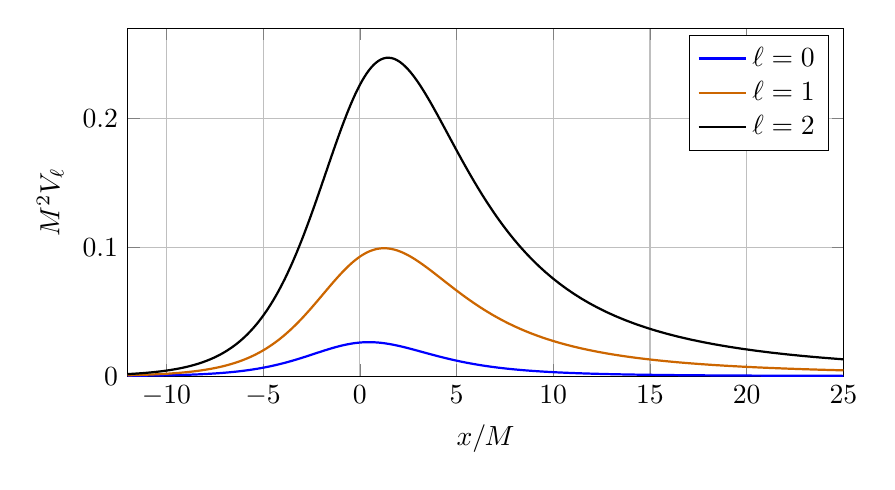
\begin{tikzpicture}
\begin{axis}[width=.88\textwidth,height=6cm,
 xlabel={$x/M$},ylabel={$M^2V_\ell$},xmin=-12,xmax=25,ymin=0,ymax=.27,
 legend style={at={(.98,.98)},anchor=north east},samples=240,
 domain=-8:3,grid=major]
% Parameterise with r = 2 + exp(z), so the horizon-side curve is resolved.
\addplot[blue,thick] ({2+exp(x)+2*(x-ln(2))},
 {exp(x)/(2+exp(x))*(2/(2+exp(x))^3)});
\addlegendentry{$\ell=0$}
\addplot[orange!80!black,thick] ({2+exp(x)+2*(x-ln(2))},
 {exp(x)/(2+exp(x))*(2/(2+exp(x))^2+2/(2+exp(x))^3)});
\addlegendentry{$\ell=1$}
\addplot[black,thick] ({2+exp(x)+2*(x-ln(2))},
 {exp(x)/(2+exp(x))*(6/(2+exp(x))^2+2/(2+exp(x))^3)});
\addlegendentry{$\ell=2$}
\end{axis}
\end{tikzpicture}
\caption{Analytic potentials evaluated from~\eqref{eq:master}, not from a
wave simulation.}
\end{figure}

\subsection{A numerically stable coordinate inversion}
The grid is uniform in $x$ on each level but needs $r(x)$ for $V$.
Directly iterating on $r-2M$ loses precision near the horizon: $r$ can round
to $2M$ even while a small positive $f$ matters. Instead set
\begin{equation}
 z=\log(r/(2M)-1),\qquad s=x/(2M)-1.
\end{equation}
Solve the monotone scalar equation
\begin{equation}\label{eq:loginverse}
 e^z+z=s,\qquad F'(z)=e^z+1>0.
\end{equation}
There is exactly one real root. Start with $z=s$ for $s\leq0$ and
$z=\log(1+s)$ otherwise. Newton's update is
\begin{equation}
 z_{\rm new}=z-\frac{e^z+z-s}{e^z+1}.
\end{equation}
Check a scaled residual and an iteration cap. Use a safeguarded root solve
if extending the coordinate range demands it. Evaluate
\begin{equation}
 q=e^z,\qquad r=2M(1+q),\qquad f=\frac{q}{1+q}.
\end{equation}
The last expression avoids subtracting nearly equal numbers. On the default
domain $x/M\in[-200,300]$, $z$ is within the range of double-precision
exponentials.

\begin{exercise}
Verify both potential limits. Test the inversion residual across the
domain using Eq.~\eqref{eq:loginverse}; near the horizon a logarithm of
the rounded $r-2M$ is not a reliable check.
\end{exercise}

\section{Initial data, characteristics and boundaries}\label{sec:initial}

The wave equation needs both $\psi$ and $\psi_t$ initially. Define the code
variable $\Pi=\pd_t\psi$. For $V=0$,
\begin{equation}
 \psi=F(x-t)+G(x+t),\qquad
 \Pi=-F'(x-t)+G'(x+t).
\end{equation}
$F$ moves towards increasing $x$, and $G$ towards decreasing $x$.
An initially incoming Gaussian is
\begin{align}\label{eq:gaussian}
 \psi(0,x)&=A\exp[-(x-x_0)^2/(2\sigma^2)],\\
 \Pi(0,x)&=\pd_x\psi(0,x)=-\frac{x-x_0}{\sigma^2}\psi(0,x).
\end{align}
For $V\ne0$ this selects the initially incoming characteristic combination;
the potential subsequently distorts and scatters the pulse. It is not an
exact translating solution on the curved background.

To see the signs, introduce $Q=\psi_x$:
\begin{equation}
 \Pi_t=Q_x-V\psi,\qquad Q_t=\Pi_x.
\end{equation}
In the free problem $\Pi+Q$ travels left and $\Pi-Q$ travels right.
The potential is a lower-order source, so it does not change the speeds
$\pm1$.

\subsection{Physical radiation conditions}
Near the future horizon the signal is ingoing. In the asymptotic regions,
\begin{equation}\label{eq:physicalbc}
 (\pd_t-\pd_x)\psi\simeq0\quad(x\ll0),\qquad
 (\pd_t+\pd_x)\psi\simeq0\quad(x\gg0)
\end{equation}
give ingoing-left and outgoing-right behaviour. At a finite outer radius
$V$ is not exactly zero, so simple Sommerfeld conditions are approximate.

\subsection{The first version's distant reflecting walls}
The initial experiment uses homogeneous Dirichlet data
$\psi(t,x_L)=\psi(t,x_R)=0$, with consistent zero time derivative.
These are reflecting computational walls. Interpret the solution only where
and when their reflected signal is negligible.

Suppose the relevant initial pulse lies in $[a,b]$. Earliest-return estimates
for an observer at $x_o$ are
\begin{equation}
 t_L=(a-x_L)+(x_o-x_L),\qquad
 t_R=(x_R-b)+(x_R-x_o).
\end{equation}
For the default pulse use $a=x_0-6\sigma=16$ and $b=x_0+6\sigma=64$.
With $x_L=-200$, $x_R=300$ and $x_o=60$, both estimates are $476$,
comfortably beyond the planned $t=200$.

The Gaussian is not compactly supported: at $6\sigma$ its amplitude is
$e^{-18}$ of its peak. Finite-difference dispersion and stencil propagation
also do not reproduce an exact continuum light cone. The estimate is a
design argument; the final check is a larger domain at identical spacing.

\begin{exercise}
Reverse the sign of $\Pi$ in a flat-space Gaussian test and predict its
trajectory. Explain why a periodic sine-wave test is useful, while periodic
boundaries would change the late-time scattering problem.
\end{exercise}

\section{Energy, flux and absorption}\label{sec:energy}

For one real mode define
\begin{equation}
 e=\frac12(\Pi^2+\psi_x^2+V\psi^2),\qquad j=-\Pi\psi_x .
\end{equation}
The background is time independent, so
\begin{align}
 \pd_t e&=\Pi(\psi_{xx}-V\psi)+\psi_x\Pi_x+V\psi\Pi\\
 &=\pd_x(\Pi\psi_x)=-\pd_x j .
\end{align}
Therefore
\begin{equation}\label{eq:energybalance}
 \frac{\dd}{\dd t}\int_{x_a}^{x_b}e\,\dd x=j(x_a)-j(x_b).
\end{equation}
Outgoing free waves have $j=\Pi^2$; incoming waves have $j=-\Pi^2$.
Positivity of $V$ makes the energy positive. With no incoming boundary flux,
the identity controls the energy of finite-energy solutions. It is not a
proof of nonlinear stability of a self-gravitating black hole.

\subsection{Relation to spacetime energy}
For a real harmonic normalised to unit angular integral, scalar Killing
energy on a Schwarzschild $t$ slice is
\begin{equation}
 E_K=\frac12\int\left[
 \Pi^2+\left(\psi_x-\frac{f\psi}{r}\right)^2
 +\frac{f\ell(\ell+1)}{r^2}\psi^2\right]\dd x .
\end{equation}
Integrating the cross term by parts gives
\begin{equation}
 E_K=\int e\,\dd x-\frac12\left[\frac{f\psi^2}{r}\right]_{x_a}^{x_b}.
\end{equation}
Thus the reduced energy agrees with the mode's physical energy when the
boundary term vanishes. The integration measure is $\dd x$, not an extra
$r^2\dd r$.

\subsection{A finite box retains the transmitted pulse}
A packet moving to very negative $x$ is approaching the horizon. At $t=200$
it may still be on our finite grid. Total reduced energy can remain nearly
constant while energy leaves the scattering region. To quantify
transmission later, integrate inward flux across a stated horizon-side
surface and account for energy left in the chosen region. A falling signal
at one observer does not measure the loss of total energy.

For real-frequency scattering on the infinite domain one can normalise
\begin{align}
 u_\omega&\sim e^{-\ii\omega x}+\mathcal R e^{+\ii\omega x}
                       &&(x\to+\infty),\\
 u_\omega&\sim\mathcal T e^{-\ii\omega x} &&(x\to-\infty).
\end{align}
The conserved Wronskian gives $|\mathcal R|^2+|\mathcal T|^2=1$ for this
real static potential with equal asymptotic wave speeds. A Gaussian has a
range of frequencies, so its reflected energy is spectrum weighted.

\begin{checkpoint}
Implement energy after the free-wave test. Check how its discrete drift
changes with resolution. Point-value AMR transfers will not conserve the
continuum energy exactly.
\end{checkpoint}

\section{Quasinormal modes and ringdown}\label{sec:qnm}

With $\psi=e^{-\ii\omega t}u_\omega(x)$,
\begin{equation}
 u_\omega''+(\omega^2-V_\ell)u_\omega=0 .
\end{equation}
A \emph{quasinormal mode} is ingoing at the future horizon and outgoing
at infinity:
\begin{equation}\label{eq:qnmconditions}
 u_\omega\sim e^{-\ii\omega x}\ (x\to-\infty),\qquad
 u_\omega\sim e^{+\ii\omega x}\ (x\to+\infty).
\end{equation}
The allowed frequencies are generally complex. Our convention is
\begin{equation}
 \omega=\omega_R-\ii\gamma,\quad\gamma>0,\qquad
 e^{-\ii\omega t}=e^{-\gamma t}e^{-\ii\omega_Rt}.
\end{equation}
The period is $2\pi/\omega_R$ and the amplitude e-folding time $1/\gamma$.

\subsection{Resonances rather than bound states}
At this complex frequency the outgoing factor grows as $e^{\gamma x}$
at the right end and the ingoing factor as $e^{-\gamma x}$ at the left.
Individual QNM eigenfunctions are not square-integrable on a constant-$t$
slice. They are resonances of an open scattering problem, not a complete
orthonormal basis of finite-energy normal modes.

The analytically continued frequency-domain retarded Green function has
resonance poles. Their residues can describe part of the time-domain signal
over an intermediate interval. Prompt propagation and late-time terms also
occur. Evolving a pulse measures that response without directly solving a
complex-frequency eigenvalue problem \cite{berti}.

\subsection{The reference for this project}
For the massless scalar, $\ell=2$, fundamental overtone $n=0$,
\begin{equation}\label{eq:reference}
 M\omega\simeq0.483644-0.096759\,\ii .
\end{equation}
This is the zero-rotation, zero-scalar-mass entry of Table~II of
Ref.~\cite{dolan}. Its period is about $12.99M$ and amplitude e-folding
time about $10.33M$. Check whether a source quotes $M\omega$ or
$2M\omega$.

The initial pulse selects an \emph{angular} mode $\ell$, not a pure radial
overtone $n=0$. It can excite several overtones and a nonresonant response.
The fundamental can dominate an intermediate interval once more strongly
damped components have decayed.

\subsection{Prompt response, ringing and tails}
Expect a transient, an interval of damped ringing, and eventually a
backscattering tail. For generic suitably localised scalar data on
Schwarzschild the familiar fixed-radius decay is $t^{-(2\ell+3)}$ under
the usual assumptions; special data or different observation limits require
care \cite{price}. Measuring a late-time tail is a later extension,
particularly sensitive to boundaries and numerical error.

\begin{exercise}
Derive the spatial growth of the asymptotic QNM factors. Explain why it
does not imply that a compact physical pulse grows without bound at large
radius.
\end{exercise}

\section{The first experiment and a defensible fit}\label{sec:experiment}

Set $M=1$, $\ell=2$, $A=1$, $x_0=40$, $\sigma=4$ and $x_{\rm obs}=60$.
Evolve to $t=200$. A rough barrier-scattering arrival estimate is
\begin{equation}
 t_{\rm arrival}\sim(x_0-x_{\rm peak})+(x_{\rm obs}-x_{\rm peak}).
\end{equation}
It suggests inspecting around $t\sim100$ and later, but does not select the
fitting window.

At the fixed observer fit
\begin{equation}\label{eq:fit}
 \psi_{\rm fit}(t)=e^{-\gamma(t-t_0)}
 [A_c\cos(\omega_R(t-t_0))+A_s\sin(\omega_R(t-t_0))].
\end{equation}
For a selected start time $t_0$, fit $A_c,A_s,\omega_R,\gamma$.
The sine/cosine form avoids a phase-wrap parameter. Estimate initial values
from the signal instead of forcing the reference into the answer.

Vary both endpoints. Early windows include prompt response and overtones;
late ones can include tails, boundaries and roundoff-dominated samples.
Inspect residuals and seek a region of stable parameters. Repeat at higher
resolution and on a larger domain. A small least-squares covariance matrix
does not describe these systematic errors; deterministic time samples are
not independent noisy measurements.

The proposed targets are errors below $1\%$ in $\omega_R$ and $3\%$ in
$\gamma$, supported by those checks. They are future acceptance goals,
not accuracy already achieved.

\begin{checkpoint}
Plot the signed waveform and a logarithmic amplitude plot before fitting.
Save raw data and exact inputs so every figure can be regenerated.
\end{checkpoint}

\section{Method of lines: from a PDE to a C++ kernel}\label{sec:mol}

Store two point values at each cell centre:
\begin{equation}
 U_i=\begin{pmatrix}\psi_i\\\Pi_i\end{pmatrix},\qquad
 x_i=x_L+(i+\tfrac12)h .
\end{equation}
The method of lines discretises space first:
\begin{equation}\label{eq:mol}
 \frac{\dd U_i}{\dd t}=\mathcal L_h(U)_i
 =\begin{pmatrix}\Pi_i\\D_{xx}\psi_i-V_i\psi_i\end{pmatrix}.
\end{equation}
This is a coupled ODE system. The background potential $V_i$ is time
independent, so calculate it when a grid is created, not at every RK stage.

\subsection{Deriving the fourth-order stencil}
Use a symmetric five-point approximation
\begin{equation}
 D_{xx}\psi_i=\frac{a\psi_i+b(\psi_{i-1}+\psi_{i+1})
                   +c(\psi_{i-2}+\psi_{i+2})}{h^2}.
\end{equation}
Taylor expansion and matching the constant, second-derivative and
fourth-derivative terms require
\begin{equation}
 a+2b+2c=0,\qquad b+4c=1,\qquad b+16c=0 .
\end{equation}
Thus $a=-5/2$, $b=4/3$, $c=-1/12$, giving
\begin{align}\label{eq:stencil}
 D_{xx}\psi_i
 &=\frac{-\psi_{i+2}+16\psi_{i+1}-30\psi_i+
                    16\psi_{i-1}-\psi_{i-2}}{12h^2}\\
 &=\psi_{xx}(x_i)-\frac{h^4}{90}\psi^{(6)}(x_i)+\OO(h^6).
\end{align}
Two neighbours on either side are needed. At block boundaries these are
supplied through \emph{ghost cells}. Never read unfilled ghosts.

These fields are point samples, not finite-volume cell averages. Both
representations are useful, but their high-order interpolation and
restriction operators differ. Preserve the point-value convention in AMR.

\subsection{RK4}
For $\dot U=\mathcal L_h(U)$, a step of size $\Delta t$ is
\begin{align}
 k_1&=\mathcal L_h(U^n),&
 k_2&=\mathcal L_h(U^n+\tfrac12\Delta t\,k_1),\\
 k_3&=\mathcal L_h(U^n+\tfrac12\Delta t\,k_2),&
 k_4&=\mathcal L_h(U^n+\Delta t\,k_3),\\
 U^{n+1}&=U^n+\frac{\Delta t}{6}(k_1+2k_2+2k_3+k_4).
\end{align}
Each stage has a temporary state. Fill that state's ghost cells before
evaluating the RHS. Updating an input array while neighbours still read it
creates a race or an unintended discretisation.

\begin{exercise}
Derive the leading truncation error in~\eqref{eq:stencil}. Write pseudocode
listing every state, temporary and ghost fill for one RK4 step. Identify
which arrays are read-only in each kernel.
\end{exercise}

\section{Stability, dispersion and boundary closures}\label{sec:stability}

\subsection{Fourier analysis on a uniform periodic grid}
For $\psi_i=e^{\ii kih}$ and $V=0$, the stencil's symbol is
\begin{equation}
 \widehat D_{xx}(k)=-\frac4{h^2}\sin^2\left(\frac{kh}{2}\right)
     \left[1+\frac13\sin^2\left(\frac{kh}{2}\right)\right].
\end{equation}
The semidiscrete frequency is $\omega_h=\sqrt{-\widehat D_{xx}}$.
It agrees with $|k|$ for well-resolved waves but differs at finite $kh$.
This numerical dispersion produces phase error. A stable run can still
have the wrong phase.

For the scalar ODE $\dot y=\lambda y$, RK4 has stability polynomial
\begin{equation}
 R(z)=1+z+\frac{z^2}{2}+\frac{z^3}{6}+\frac{z^4}{24}.
\end{equation}
On the imaginary axis,
\begin{equation}
 |R(\ii y)|^2=1-\frac{y^6}{72}+\frac{y^8}{576},
\end{equation}
so $|y|\leq2\sqrt2$ is the relevant stable interval. Since
$\omega_{h,\max}^2=16/(3h^2)$, the free periodic problem requires
\begin{equation}
 \frac{\Delta t}{h}\leq\sqrt{\frac32}.
\end{equation}
Start conservatively at $\Delta t=0.2h$.
For constant positive $V$, $\omega_h^2=-\widehat D_{xx}+V$.
A useful bound for the symmetric uniform-grid operator with bounded
$V\geq0$ is
\begin{equation}
 \Delta t\lesssim
 \frac{2\sqrt2}{\sqrt{16/(3h^2)+V_{\max}}}.
\end{equation}
This is not a stability proof for a changing AMR hierarchy with boundary
interpolation. Large $\ell$ increases $V_{\max}$. Check new regimes
rather than assuming the initial CFL number covers all parameters.

\subsection{Cell-centred endpoint data}
The first valid point is $x_L+h/2$, a half-cell from the left boundary face.
Homogeneous Dirichlet data can be imposed by odd reflection:
\begin{equation}
 \psi_{-1}=-\psi_0,\quad\psi_{-2}=-\psi_1,\qquad
 \Pi_{-1}=-\Pi_0,\quad\Pi_{-2}=-\Pi_1 .
\end{equation}
At the right face of a grid with valid indices $0,\ldots,N-1$,
\begin{equation}
 \psi_N=-\psi_{N-1},\qquad\psi_{N+1}=-\psi_{N-2},
\end{equation}
and similarly for $\Pi$. This places zero at the face, not the first
cell centre. It is a reflecting closure, not a radiation condition.
Domain enlargement checks its relevance to our finite-time experiment.

\begin{checkpoint}
The first numerical result should be the exact periodic wave
$\psi(t,x)=\sin(x-t)$, $\Pi(t,x)=-\cos(x-t)$ on $[0,2\pi]$.
Establish convergence of the complete space-and-time scheme before adding
the black-hole potential.
\end{checkpoint}

\section{Adaptive meshes without losing the numerical problem}\label{sec:amr}

Use $a=0,1,\ldots$ for refinement levels and $\ell$ for angular modes.
With refinement ratio two,
\begin{equation}
 h_a=h_0/2^a.
\end{equation}
Fine patches replace the effective solution in selected coarse regions.
Both representations may remain allocated, but they are not two physical
copies of the same volume.

\subsection{Four different operations}
\begin{description}[style=nextline]
\item[Same-level ghost exchange.]
Copy data across neighbouring boxes, including periodic neighbours.
\item[Prolongation.]
Interpolate coarse data to fine ghost points or new fine grids.
For this point-value scheme use the tutorial's quartic spatial interpolation.
\item[Restriction.]
Synchronise coarse data from the finer representation. Use the tutorial's
fourth-order point-value restriction. Simple volume averaging has different
semantics and can reduce this scheme's order.
\item[Regridding.]
Choose a new hierarchy, transfer data, rebuild grid-dependent quantities
and masks, and discard obsolete patches at supported synchronised times.
\end{description}

\subsection{Time subcycling is an interpolation problem too}
A ratio-two fine level can take two steps while its parent takes one.
Fine RK stages need parent boundary information at intermediate times.
Linear interpolation between parent endpoints is generally insufficient
for fourth-order evolution. AMReX's \code{AmrLevel::RK} and associated
fill-patching machinery support RK-aware coarse/fine time handling.
Follow the official wave tutorial's pattern \cite{wave}, then test it.

Progress through a single level, a fixed refined patch, subcycling and
dynamic regridding. If an interface emits a small reflected pulse in a
flat-wave test, measure how its amplitude changes with refinement. It
must not be mistaken for black-hole scattering.

\subsection{A first tagging rule}
Always refine $[-20,80]$ on levels eligible for further refinement.
It contains the potential barrier, initial pulse and observer.
Outside it, start with
\begin{equation}
 \eta_i=\frac{h_a^2|D_{xx}\psi_i|}
             {\max(\max_{\text{valid on }a}|\psi|,10^{-12})}.
\end{equation}
Tag where $\eta_i>10^{-3}$, add eight buffer cells, and regrid every
four coarse steps. These are initial experimental choices.
The indicator is a curvature heuristic, not a rigorous fourth-order error
estimator. It can miss features of another variable or be affected by a
large amplitude elsewhere. Sweep the threshold and compare to a uniform
reference.

The forced interval also prevents the decaying ringdown from losing all
local refinement as its amplitude shrinks. All indicators must use valid,
appropriately filled data.

\subsection{Composite integrals}
Let $m_{a,i}=1$ for a valid cell not covered by a finer level and zero
otherwise. Then
\begin{equation}\label{eq:composite}
 E_h=\sum_{a,i}m_{a,i}h_a e_{a,i}
\end{equation}
counts each region once. Exclude ghosts and rebuild masks after regridding.
Use the same convention for error norms and active-cell counts.
The equation is reduced to a Cartesian $x$ line, so the weight is $h_a$,
with no spherical Jacobian.

The point-value stencil and transfers are not an exactly conservative
finite-volume AMR method. Do not claim exact energy conservation or add
a flux register without deriving the appropriate discrete conservation law.

\section{The AMReX concepts to recognise in C++}\label{sec:amrex}

The framework supplies storage and mesh operations; your code supplies
the equations and their validation. A useful mapping is:
\begin{center}
\begin{tabularx}{\textwidth}{@{}lX@{}}
\toprule
AMReX concept & Role in this project\\
\midrule
\code{Geometry} & Physical domain, spacing and periodicity.\\
\code{Box}, \code{BoxArray} & Integer-index regions and their block decomposition.\\
\code{DistributionMapping} & Assignment of blocks to MPI ranks when enabled.\\
\code{MultiFab} & Field components and ghost storage across blocks.\\
\code{Array4} & Lightweight indexed view of a block's data.\\
\code{ParallelFor} & Cell kernels expressed for AMReX execution backends.\\
\code{FillBoundary} & Same-level and periodic ghost communication.\\
Fill-patching & Physical boundary and coarse/fine space-time preparation.\\
\code{AmrLevel} & Hooks for initial data, evolution, tagging and synchronisation.\\
\bottomrule
\end{tabularx}
\end{center}

The initial \code{main.cpp} allocates a uniform \code{MultiFab} with
two components and two ghost cells. The AMR hierarchy comes later.
Consult the official documentation and pinned tutorial for interfaces
\cite{amrex,wave,gpu}.

\subsection{Kernel and ownership discipline}
Read the stage input and potential; write a separate RHS array. Keep
per-cell arithmetic in the kernel and allocation/configuration outside.
Do not keep a view after its owner has been reallocated during regridding.
Destroy AMReX objects before \code{amrex::Finalize}.

CPU correctness comes first. Supported AMReX abstractions ease later
MPI/GPU work but do not establish backend correctness or speed.
Compare results after enabling each backend.

\subsection{Performance measurements}
Count active cells and actual RHS cell updates across levels and RK stages.
Measure total runtime and, later, time in RHS kernels, ghost filling,
regridding and I/O. Use Release builds and repeat short runs.
AMR can reduce cell updates yet increase runtime for a small 1D problem:
bookkeeping and communication carry overhead. That is a useful measurement,
not a failed result.

\section{Verification and interpretation of error}\label{sec:verification}

\subsection{Exact solutions first}
For a smooth analytic test and numerical error $e_i$, define for example
\begin{equation}
 \norm{e}_{2,h}=
 \left(\frac{\sum_i h e_i^2}{\sum_i h}\right)^{1/2},\qquad
 \norm{e}_{\infty,h}=\max_i|e_i|.
\end{equation}
Use composite masks for AMR. If $E(h)=Ch^p+\cdots$, then
\begin{equation}
 p_{\rm obs}=\log_2\frac{E(h)}{E(h/2)}
\end{equation}
approaches the method's order in the resolved regime. The complete
uniform-grid scheme should approach fourth order with $\Delta t\propto h$
and sufficiently accurate boundary and extraction treatment.

Without an exact answer compare three resolutions at common physical
times and positions. For a sampled waveform $w_h(t)$,
\begin{equation}
 p_{\rm obs}\simeq
 \log_2\frac{\norm{w_h-w_{h/2}}}{\norm{w_{h/2}-w_{h/4}}}.
\end{equation}
Interpolation to common points must not dominate the difference.
Do not divide pointwise by a waveform near its zero crossings; use a
norm over a stated interval.

\subsection{Separate the error sources}
\begin{enumerate}
\item \textbf{Space and time discretisation:} vary $h$, and independently
      reduce the CFL factor on one grid to identify time-integration effects.
\item \textbf{Finite domain:} enlarge the domain at fixed spacing.
      Increasing both size and spacing confounds two changes.
\item \textbf{AMR transfers:} compare fixed interfaces, regridding and a
      uniform mesh with the same finest spacing.
\item \textbf{Extraction:} use at least fourth-order spatial interpolation
      and test it on a known smooth function.
\item \textbf{Fit/model error:} vary the ringdown window and inspect residuals.
      A single damped sinusoid is an approximation to the full signal.
\item \textbf{Floating point:} identify when small signals or convergence
      differences reach roundoff or cancellation levels.
\end{enumerate}

\subsection{A reproducible study}
Use uniform grids of $1024$, $2048$ and $4096$ cells, with an $8192$-cell
reference on the default domain. Adaptive base grids of $256$, $512$ and
$1024$, each with two finer levels, give the corresponding finest spacings.
Matching that spacing does not make the errors identical: coarse regions
and transfers still matter.

Record input files, application and AMReX revisions, dirty-tree state,
compiler, build type and machine. Save the raw waveform and diagnostic CSVs.
Report accuracy against both runtime and cell updates. An optimisation
must preserve the stated accuracy criterion.

\begin{exercise}
Suppose halving $h$ reduces error by four, despite a fourth-order interior
stencil. Give three plausible causes and a numerical comparison that
distinguishes each one.
\end{exercise}

\section{Preparation for full numerical relativity}\label{sec:fullnr}

Full NR evolves geometry as well as matter. In a $3+1$ split,
\begin{equation}
 \dd s^2=-\alpha^2\dd t^2+
 \gamma_{ij}(\dd x^i+\beta^i\dd t)(\dd x^j+\beta^j\dd t).
\end{equation}
Here $\alpha$ is the lapse, $\beta^i$ the shift and $\gamma_{ij}$ the spatial
metric. With $K_{ij}=-\tfrac12\mathcal L_n\gamma_{ij}$, the constraints are
\begin{align}
 {}^{(3)}R+K^2-K_{ij}K^{ij}&=16\pi\rho,\\
 D_j(K^{ij}-\gamma^{ij}K)&=8\pi S^i,
\end{align}
where $\rho=T_{\mu\nu}n^\mu n^\nu$ and
$S_i=-\gamma_i{}^\mu n^\nu T_{\mu\nu}$.
The evolution additionally needs gauge choices and a suitable formulation.

On our Schwarzschild exterior slicing,
$\alpha=\sqrt f$, $\beta^i=0$, and $K_{ij}=0$ are prescribed.
We do not solve the sourced constraints: backreaction was dropped at the
chosen perturbative order. Also, $\Pi=\pd_t\psi$ is not every NR
scalar-momentum convention. For example, if
$\Pi_{\rm NR}=-n^\mu\pd_\mu\Phi$, then
\begin{equation}
 \Pi_{\rm NR}=-\frac{Y_{\ell m}}{r\sqrt f}\,\Pi .
\end{equation}
Translate definitions before borrowing equations or code.

The transferable skills are deriving an evolution system, implementing
stencils and stage-dependent boundaries, testing convergence, understanding
mesh transfers, and extracting a physical observable with defensible
uncertainty. New material in full NR includes constraint-satisfying initial
data, gauge dynamics, formulations such as BSSN or CCZ4, horizon diagnostics
and matter backreaction.

Extensions after the core result include outgoing boundaries, a controlled
tail study, MPI process-count checks, or full 3D test-field evolution.
The latter requires a new spatial formulation and boundary design; running
the radial code on a cluster alone does not provide those ingredients.

\appendix
\section{Conventions at a glance}
\begin{center}
\begin{tabularx}{\textwidth}{@{}lX@{}}
\toprule
Quantity & Meaning\\
\midrule
$M$ & Schwarzschild mass; one in the numerical inputs.\\
$r$ & Areal radius, $r>2M$.\\
$x$ & Tortoise coordinate with the constant of Eq.~\eqref{eq:tortoise}.\\
$t$ & Schwarzschild coordinate time used for waveforms.\\
$\Phi$ & Full classical scalar field.\\
$\psi$ & Reduced mode: $\Phi=\psi Y_{\ell m}/r$.\\
$\Pi$ & Code variable $\pd_t\psi$.\\
$\ell,m$ & Angular indices, distinct from refinement level $a$.\\
$n$ & QNM overtone; the reference targets $n=0$.\\
$\omega_R-\ii\gamma$ & QNM frequency with time dependence $e^{-\ii\omega t}$.\\
$h_a$ & Spacing at refinement level $a$.\\
$e,j$ & Reduced energy density and right-directed flux.\\
\bottomrule
\end{tabularx}
\end{center}

\clearpage
\section{Questions to bring to a code review}
\begin{enumerate}
\item Derive the radial equation and identify every approximation.
\item Explain the horizon-side signs in the initial momentum and harmonic
      boundary condition.
\item Derive and test the logarithmic coordinate inversion.
\item Derive the stencil and periodic-grid RK4 stability bound.
\item Demonstrate exact travelling-wave convergence.
\item Explain ghost filling at RK stages and refinement interfaces.
\item Derive the energy balance including boundary flux.
\item Show how composite integrals count each region once.
\item Explain your fitting window and separate numerical from fitting error.
\item State which ingredients of nonlinear Einstein evolution remain to learn.
\end{enumerate}

\begin{thebibliography}{9}
\bibitem{berti}
E.~Berti, V.~Cardoso and A.~O.~Starinets,
\emph{Quasinormal modes of black holes and black branes},
Class.\ Quantum Grav.\ \textbf{26}, 163001 (2009),
\href{https://arxiv.org/abs/0905.2975}{arXiv:0905.2975v2}.
Read the perturbation primer and QNM boundary conditions first; the entire
review is not a prerequisite.

\bibitem{dolan}
S.~R.~Dolan,
\emph{Instability of the massive Klein--Gordon field on the Kerr spacetime},
Phys.\ Rev.\ D \textbf{76}, 084001 (2007),
\href{https://arxiv.org/abs/0705.2880}{arXiv:0705.2880}.
Table II at zero rotation and zero scalar mass supplies the reference.

\bibitem{price}
R.~H.~Price,
\emph{Nonspherical Perturbations of Relativistic Gravitational Collapse.
I. Scalar and Gravitational Perturbations},
Phys.\ Rev.\ D \textbf{5}, 2419 (1972),
\href{https://doi.org/10.1103/PhysRevD.5.2419}{doi:10.1103/PhysRevD.5.2419}.
Background for the tail extension.

\bibitem{amrex}
AMReX developers, \emph{AMReX documentation},
\href{https://amrex-codes.github.io/amrex/docs_html/}{official documentation}.
The project pins release 26.09, commit
\href{https://github.com/AMReX-Codes/amrex/tree/a52ca73324ac2c7b65ec04f131e6df99eec9c576}
{\texttt{a52ca73324ac}}. Online development documentation can differ.

\bibitem{wave}
AMReX developers, \emph{Wave\_AmrLevel tutorial},
\href{https://github.com/AMReX-Codes/amrex-tutorials/tree/1a73f32e10514d917333ea7a3fd54e661e232144/ExampleCodes/Amr/Wave_AmrLevel}
{pinned source at \texttt{1a73f32e1051}}.
Reference for point values, RK-aware evolution, interpolation and restriction.
Its reflecting boundaries must be interpreted for the chosen experiment.

\bibitem{gpu}
AMReX developers, \emph{Overview of AMReX GPU support},
\href{https://amrex-codes.github.io/amrex/docs_html/GPU.html}
{official documentation}.
Reference for portable kernels and reductions; GPU execution is a later
extension. External sources checked 12 September 2026.
\end{thebibliography}
\end{document}
